\documentclass{udpreport}
\documentclass{article}
\usepackage[export]{adjustbox}
\title{Comprobación del funcionamiento del algoritmo STP e implementación de VLAN}
\author{Integrantes: Thomas Muñoz, Ignacio Yanjari, Dagoberto Navarrete, Ignacio López.}
\date{19 de Mayo de 2016}
\usepackage{graphicx}
\usepackage{float}
\graphicspath{ {images/} }
\udpschool{Escuela de Informática y Telecomunicaciones}

\begin{document}
\maketitle
\tableofcontents
\listoffigures
\chapter{Introducción}
  En este laboratorio se comprobara el funcionamiento del protocolo STP (IEEE 802.1D),  esto se llevara a cabo gracias al uso del programa CISCO Packet Tracer, también se implementara el protocolo de  VLAN (IEEE 802.1Q), de esta manera podremos entender cómo funciona, qué  ventajas tiene, y como implementarlo de manera eficiente.
\chapter{Actividades}
	\section{Topología base con bucles}
	Primero se procede a abrir el programa CISCO Packet Tracer, desde la consola del equipo del laboratorio, una vez hecho esto se
	continúa a sacar tres switch desde la parte inferior izquierda en el apartado de switch, después se posicionan de manera que
	formen un triángulo y así formen una topología con bucles.\\\\
	\begin{figure}[H]
    \centering
    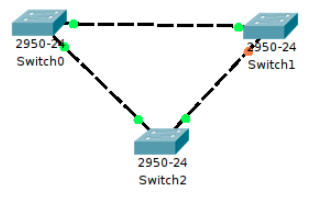
\includegraphics[width=8cm]{act1}
    \caption{Topología con bucles}
    \end{figure}
    
	{\large \bf{Cuestionario: }}\\
	\begin{enumerate}
	    \item ¿Qué camino realizara un paquete que para llegar desde el switch
                0 hasta el switch2?\\\\
                 Como el protocolo STP no afectó al enlace entre estos switches, el paquete se envía de forma directa sin pasar por otro switch.
    
        \item ¿Qué camino realizara un paquete que para llegar desde el switch
            2 hasta el switch1?\\\\
            Como el protocolo STP afectó al enlace entre estos switches dejando el puerto que va desde el switch 1 al switch 2 como bloqueado. El camino recorrido por el paquete será: Switch 2 - Switch 0 - Switch 1.\\\\\\\\\\\ 
	\end{enumerate}
	\section{Configuración de STP}
	Una vez con la topología con bucles se procede a aplicarle el protocolo STP, para llevar esto acabo se deberá configurar cada
	switch desde la consola, esto se realiza haciendo clic en el switch, después se va a la pestaña donde dice CLI, y ahí se le
	ingresan los comandos correspondientes para configurar cada switch según sea necesario. Se configura un switch como
	primario y los otros dos como secundarios.\\
	\begin{figure}[H]
	\centering
	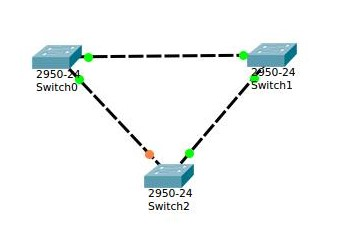
\includegraphics[width=8cm]{act2}
	\caption{Topología con roots asignados}
	\end{figure}\\
    \begin{enumerate}
	    \item ¿Qué camino realizará un paquete que para llegar desde el switch
2 hasta el switch0?\\\\
        Como el protocolo STP afectó al enlace entre estos switches dejando el puerto que va desde el switch 2 al switch 0 como bloqueado. El camino recorrido por el paquete será: Switch 2 - Switch 1 - Switch 0. 
        \item  ¿Qué camino realizará un paquete que para llegar desde el switch
1 hasta el switch0?\\\\
          Como el protocolo STP no afectó al enlace entre estos switches, el paquete se envía de forma directa sin pasar por otro switch.
	\end{enumerate}
	\section{Priorización STP}
	   
	    Ya aplicada la configuración del STP se continua a asignarle una prioridad a cada switch,  para esto nuevamente se hace clic	sobre él, y luego se dirige hacia la pestaña CLI, ya una vez ahí se le asigna la prioridad a cada switch con el comandocorrespondiente, al switch0 se le asigna prioridad 2, el switch 1 prioridad 1, mientras que al switch2 no se le asigna prioridad.\\
	
	\section{Configuración VLAN}
	    Para realizar esta actividad primero se armara una topología idéntica a la que se entrega, para esto se sacaran 6 switch, y 8 equipos, una vez ubicándolos bien en el espacio se procede a configurar cada VLAN, para que esto se lleve a cabo primero se deberá agregar cada VLAN a cada switch correspondiente, esto se hace directamente en la consola de cada switch, luego se configurar la puerta de red, la cual puede estar en modo Access o en modo Trunk, se utilizara el modo Access cuando se trate de una sola VLAN que transitara por ahí, por el contrario si van a transitar muchas VLAN se deberá configurar en modo Trunk.\\\\
    Para finalizar y comprobar que la configuración este correcta se realiza un ping desde cada equipo y se observa que cada
	paquete le llegue solo a los equipos pertenecientes a la misma VLAN.\\
	
	{\large \bf{Cuestionario: }}\\
	\begin{enumerate}
	    \item ¿Cuál es la diferencia del modo Access y el modo Trunk en un switch?\\\\
	         El modo Trunk se utiliza para configurar las conexiones de switch a switch, indicando las vlan que pueden pasar por ese enlace. Por otro lado el modo Access es para conexiones desde el switch a un host, para indicar la vlan que puede pasar por el canal (por lo general es la misma vlan a la que pertenece el host).
        \item  ¿Qué ocurre si conecto una puerta en modo Trunk a un PC?\\\\
            Llegarían al PC todos los paquetes provenientes de las VLAN permitidas en la configuración del modo Trunk del respectivo puerto.
        \item ¿Qué ocurre si conecto dos switches, uno en modo access y otro en modo trunk?\\\\
              Transmitirían entre ellos solo los paquetes pertenecientes a la VLAN 
  	      permitida en el Switch configurado en modo Access.
  	     \item  ¿Qué camino realizara un paquete que para llegar desde el switch 1 hasta el switch 0?\\\\
  	     
	\end{enumerate}
\chapter{Conclusión}
  	     
  	      
 %MODIFICAR BIBLIOGRAFÍA ENTERA !! APRENDAN LATEX ! gg wp
\begin{thebibliography}{x}
\bibitem{Scapy Documentation} \textsc{Scapy Documentation},
\textit{http://www.secdev.org/projects/scapy/files/scapydoc.pdf}
\bibitem{Cisco Osi} \textsc{Cisco},
\textit{ http://www.cisco.com/cpress/cc/td/cpress/fund/ith/ith01gb.htm#xtocid166844}
\end{thebibliography}
% -----------------------------------------------------------------------------------------------
\end{document}
